\section{Results and Discussion}

\subsection{Hybrid Film Growth and Thickness Control}

Hybrid organic--inorganic thin films were deposited via molecular layer deposition (MLD) using trimethylaluminum (TMA) or diethylzinc (DEZ) with bifunctional organic diol precursors. Growth per cycle (GPC) values ranged from approximately \SI{1}{\angstrom\per\cycle} to \SI{6}{\angstrom\per\cycle}, consistent with controlled, stoichiometric MLD growth and avoidance of chemical vapor deposition (CVD)-like behavior~\cite{Wang2022}.

Alucone films (TMA-based) consistently exhibited higher GPCs than zincone films (DEZ-based) across all organic linkers, typically between \SIrange{3}{6}{\angstrom\per\cycle}. Among these, alucones synthesized with 1,4-butynediol (BTY) achieved the highest GPCs (up to \SI{6}{\angstrom\per\cycle}), attributed to the rigidity and linear geometry imposed by the internal carbon--carbon triple bond. This structural constraint likely enhances monolayer formation by reducing conformational flexibility and improving surface reactivity~\cite{Smith2023}. Intermediate GPC values were observed for alucones formed from cis-2-butene-1,4-diol (CB), 2-methylene-1,3-propanediol (MPD), and 1,3,5-trihydroxybenzene (THB), reflecting the influence of steric bulk, branching, and aromaticity on saturation behavior.

Zincone films exhibited lower and more variable GPCs (\SIrange{1}{4}{\angstrom\per\cycle}), which may stem from less favorable adsorption dynamics or weaker Zn--O--C bonding~\cite{Zhao2023}.\footnote{Citation to be confirmed.} However, these values are likely underestimated due to post-deposition hydrolysis and partial film loss prior to ellipsometric measurement. This phenomenon is discussed further in Section~\ref{sec:stability}.

Final film thicknesses were tuned between \SIrange{20}{80}{\nano\meter} by varying the number of MLD cycles (typically 100). Spectroscopic ellipsometry confirmed high uniformity and reproducibility across batches (Supplementary Figure~S1), validating the MLD process as a robust and scalable platform for subsequent evaluations.

\subsection{Air Stability and Degradation Resistance}

The environmental stability of hybrid films was evaluated by monitoring changes in thickness after ambient air exposure at \SI{20}{\celsius} and \SIrange{40}{50}{\percent} relative humidity for \SI{1}{\hour} and \SI{24}{\hour}. Thicknesses were measured by spectroscopic ellipsometry.

Zincone films exhibited rapid and severe degradation, losing over 40\% of their thickness within the first \SI{10}{\minute}. This pronounced instability is attributed to the hydrolytic vulnerability of Zn--O--C bonds, due to the electrophilicity of zinc centers and the relatively weak coordination compared to aluminum-based analogues~\cite{Nguyen2023}. Ultraviolet (UV) exposure at \SI{254}{\nano\meter} modestly slowed degradation rates, but significant thickness loss still occurred over \SI{24}{\hour}, especially for films based on ethylene glycol (EG), 2-methylene-1,3-propanediol (MPD), and 3,4-dihydroxy-1-butene (DHB).

In contrast, alucone films demonstrated superior air stability. As-deposited alucones showed moderate thickness reductions (\SIrange{10}{20}{\percent}) over \SI{24}{\hour}, whereas UV-treated alucones retained over 95\% of their original thickness. This enhancement is attributed to UV-induced crosslinking and network densification, which reduce moisture access to reactive sites~\cite{Park2025}.

These results underscore the critical role of metal center identity and crosslink density in determining environmental robustness. The strong contrast in degradation behavior between zincones and alucones supports the selection of aluminum-based hybrid networks for further lithographic development.

\begin{figure}[H]
  \centering
  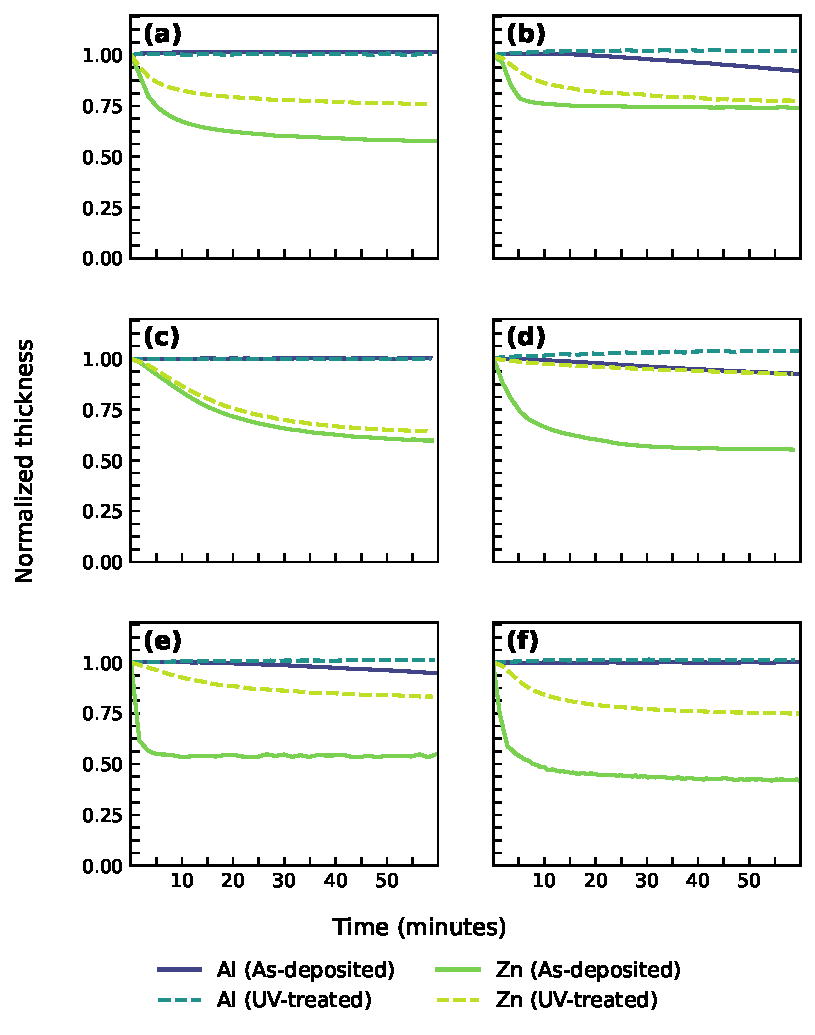
\includegraphics[width=0.75\textwidth]{Figures/air_stability_final.pdf}
  \caption{\small
    Normalized thickness change over 1 hour of air exposure for Al-based and Zn-based hybrid thin films incorporating different organic linkers. (a) MPD (methylenepropanediol); (b) EG (ethylene glycol); (c) THB (trihydroxybenzene); (d) BTY (1,4-butynediol); (e) DHB (dihydroxybutene); (f) CB (cis-butenediol).
    Solid lines represent as-deposited films, while dashed lines correspond to UV-treated films. Aluminum-based (Al) and zinc-based (Zn) films are distinguished by color. Thickness values were normalized to the initial thickness at time zero.
  }
  \label{fig:air_stability}
\end{figure}

\subsection{Developer Compatibility and Patterning Contrast}

Chemical robustness was evaluated by immersing hybrid films in DI water, anhydrous organic solvents (acetone, toluene, chloroform), and dilute aqueous developers (\SI{0.01}{\molar} HCl and \SI{0.01}{\molar} KOH) for \SI{1}{\hour}. Post-treatment thicknesses and refractive indices were measured via spectroscopic ellipsometry.

Zincone films showed extreme sensitivity, rapidly dissolving in aqueous media and undergoing substantial degradation in organic solvents. This instability is consistent with the facile hydrolytic cleavage of Zn--O--C linkages upon exposure to moisture and polar solvents~\cite{King2009}. Although UV pretreatment provided modest improvements in handling stability, the inherent chemical fragility of zincones limited their viability for lithographic applications.

In contrast, alucone films displayed significantly greater chemical resistance. As-deposited alucones lost \SIrange{10}{20}{\percent} thickness in DI water, indicative of partial hydrolysis. Organic solvents produced minor thickness increases and decreases in refractive index, likely due to limited solvent uptake and the formation of porous domains within the film~\cite{Vemuri2008}. UV-treated alucones retained both thickness and refractive index across all solvents and aqueous developers, reflecting their densified and crosslinked structure.

Three visualization formats were used to compare etch stability: (a) heatmaps of organic linker vs. solvent, (b) grouped bar charts with solvents on the x-axis and linkers grouped by color, and (c) grouped bar charts with linkers on the x-axis and solvents grouped by color. Organic linkers are ordered by chemical structure: EG (ethylene glycol), CB (cis-butenediol), BTY (butynediol), THB (trihydroxybenzene), MPD (methylenepropanediol), and DHB (dihydroxybutene). Solvents are ordered from aqueous (\SI{0.01}{\molar} HCl, \SI{0.1}{\molar} KOH, water, ethanol) to polar aprotic (acetone) to nonpolar (chloroform, toluene). A consistent y-axis range was used to allow visual comparison between Al- and Zn-based films. Colors correspond to exposure condition using the Viridis colormap.

While both \SI{0.01}{\molar} HCl and KOH fully removed the films with extended immersion, KOH was excluded from further development studies due to its aggressive etching of silicon substrates and risk of undercutting~\cite{Horie2010}. HCl enabled selective removal of unexposed regions via protonation and hydrolysis of metal--O--C bonds, making it the preferred developer.

Short-time immersion tests in \SI{0.01}{\molar} HCl showed strong contrast between as-deposited and UV-treated alucones. UV treatment significantly delayed dissolution, enabling high-resolution patterning. This strong contrast informed the selection of alucone materials for subsequent electron-beam lithography (EBL) evaluation.

\begin{figure}[H]
  \centering

  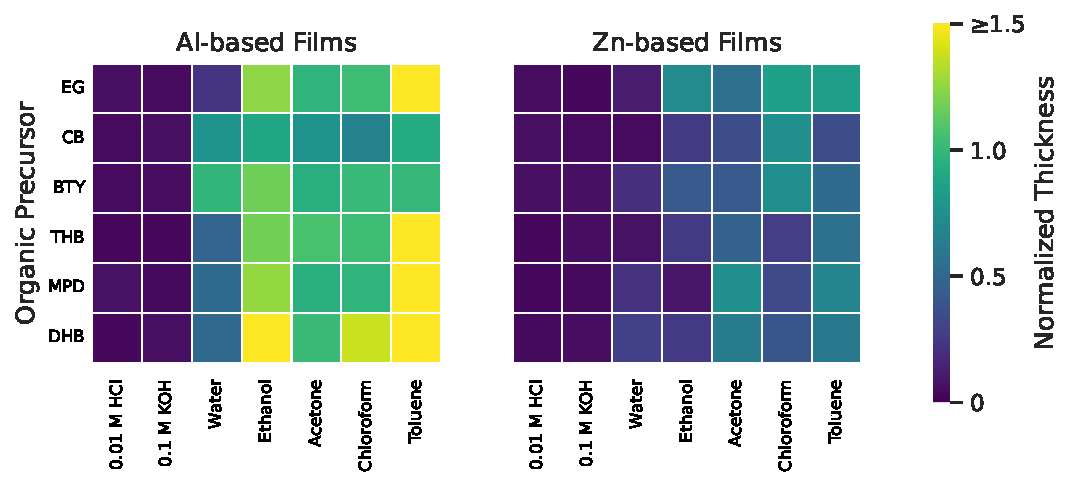
\includegraphics[width=0.9\textwidth]{Figures/Fig4a_Heatmap_EtchStability.pdf}
  \vspace{1em}

  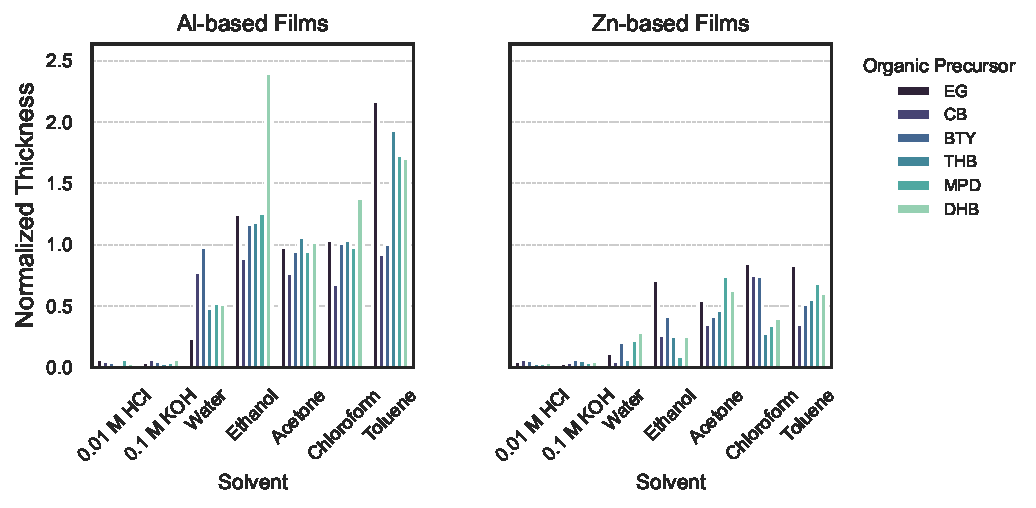
\includegraphics[width=0.9\textwidth]{Figures/Fig4b_Barplot_EtchStability.pdf}
  \vspace{1em}

  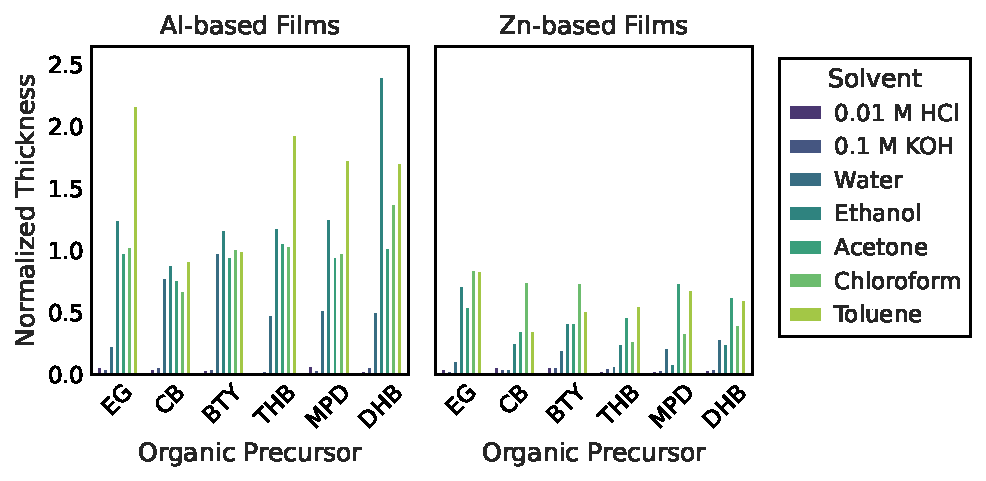
\includegraphics[width=0.9\textwidth]{Figures/Fig4c_BarplotOrganicGroupedBySolvent.pdf}

  \caption{
    Normalized thickness of as-deposited hybrid films after \SI{1}{\hour} solvent immersion, shown using three complementary visualization formats:
    \textbf{(a)} heatmaps of organic linker vs. solvent for Zn- and Al-based hybrid films (DEZ and TMA precursors, respectively);
    \textbf{(b)} grouped bar charts with solvents on the x-axis and organic linkers grouped by color; and
    \textbf{(c)} grouped bar charts with organic linkers on the x-axis and solvents grouped by color.
    Organic linkers are ordered by chemical structure: EG (ethylene glycol), CB (cis-butenediol), BTY (butynediol), THB (trihydroxybenzene), MPD (methylenepropanediol), and DHB (dihydroxybutene).
    Solvents are ordered from aqueous (\SI{0.01}{\molar} HCl, \SI{0.1}{\molar} KOH, water, ethanol) to polar aprotic (acetone), and nonpolar (chloroform, toluene).
  }
  \label{fig:developer_visualization_comparison}
\end{figure}

\subsection{Selection of Lead Materials for Advanced Characterization}

The results of air stability and chemical compatibility studies guided the selection of alucone films for further structural and spectroscopic characterization. The goal was to identify systems that not only exhibit UV-induced transformation but also demonstrate environmental robustness suitable for patterning applications.

Zincone films were excluded early due to their severe chemical instability under ambient and aqueous conditions. Their rapid hydrolysis, combined with concerns over zinc volatility and potential contamination under vacuum, made them unsuitable for further development~\cite{Richey2019}.

Among the alucones, BTY-based films stood out for their high and consistent growth per cycle (\SI{\sim 6}{\angstrom\per\cycle}) and pronounced UV-induced chemical changes observed by both FTIR and XPS. These included the disappearance of hydroxyl features, emergence of conjugated C=C and C=O signals, and reduced susceptibility to hydrolysis, indicative of robust photochemical crosslinking. As a result, BTY was selected for detailed spectroscopic analysis and electron-beam lithography (EBL) evaluation.

THB-based alucones also exhibited good environmental stability, even without UV treatment. However, their FTIR and XPS spectra showed only subtle changes upon UV exposure, with limited evidence of crosslinking or significant structural reorganization. Due to this lack of responsiveness to UV activation, THB films were not advanced to lithographic testing. Still, their aromaticity and partial degradation resistance justified their inclusion as a chemically stable control for extended spectroscopic analysis.

Other organic linkers, such as CB and MPD, were deprioritized. CB-based films showed moderate UV-induced stabilization but fell short of the crosslinking efficiency observed in BTY. MPD-based films exhibited minimal chemical change with UV exposure and poor aqueous stability, indicating limited suitability for further development.

In summary, BTY and THB alucones were selected as lead candidates for advanced FTIR and XPS characterization. BTY-based films were prioritized for lithography due to their strong UV response and structural transformation, while THB-based films served as a stable aromatic control to explore the boundaries of UV-induced network modification.

\subsection{FTIR Analysis: UV-Induced Crosslinking and Network Densification}

Fourier-transform infrared (FTIR) spectroscopy was used to analyze the chemical and structural changes induced by ultraviolet (UV) exposure (\SI{254}{\nano\meter}) in TMA–BTY alucone films. Spectra acquired before and after UV irradiation revealed clear modifications in vibrational modes associated with hydroxyl, carbon–carbon, and metal–oxygen bonding environments, providing mechanistic insight into crosslinking and network densification (Figure~\ref{fig:ftir}).

As-deposited films showed broad O–H stretching bands centered near 3622 and 3232~\si{\per\centi\meter}, corresponding to free and hydrogen-bonded hydroxyl groups, respectively. These bands were significantly diminished after UV exposure, indicating consumption of terminal –OH groups via condensation, elimination, or photochemical reactions. This is consistent with the disappearance of hydroxyl signatures in post-UV XPS and supports a densification mechanism driven by hydroxyl removal.

A key transformation was the emergence and sharpening of the band at \SI{1612}{\per\centi\meter}, attributed to C=C stretching vibrations. This suggests the formation of conjugated or aromatic domains, likely resulting from cycloaddition or radical-mediated rearrangement of BTY’s internal alkyne units. Although C≡C stretching modes were obscured by overlapping CO$_2$ features, the evolution of C=C peaks provides indirect evidence of alkyne conversion.

In the fingerprint region, characteristic Al–O–C backbone vibrations appeared between \SIrange{1200}{800}{\per\centi\meter}, including strong peaks at 1132, 1063, and 1012~\si{\per\centi\meter}, along with broader modes below 700~\si{\per\centi\meter}. Following UV exposure, these bands narrowed and sharpened, consistent with increased structural order. Al–O bending vibrations near 579 and 557~\si{\per\centi\meter} also became more defined, indicating enhanced crosslink density.

Collectively, these spectral changes support a mechanism where UV irradiation removes hydroxyl groups, induces alkyne–alkyne or alkyne–hydroxyl coupling, and promotes rearrangement into conjugated or partially aromatic structures. These transformations reduce free volume, increase cohesion, and improve resistance to hydrolysis—consistent with the enhanced film stability observed in chemical and aqueous testing.

\begin{figure}[ht]
  \centering
  \includegraphics[width=0.75\textwidth]{Figures/Fig3_FTIR_Main.pdf}
  \caption{FTIR spectra of TMA–BTY alucone films before and after UV irradiation at 254~nm. Notable changes include disappearance of O–H stretching bands (3622 and 3232~\si{\per\centi\meter}), emergence of a sharp C=C stretch near 1612~\si{\per\centi\meter}, and sharpening of Al–O–C and Al–O bending modes in the fingerprint region. These features are consistent with UV-induced crosslinking and structural densification.}
  \label{fig:ftir}
\end{figure}

\subsection{XPS Analysis of Bonding Environments and Stability}

X-ray photoelectron spectroscopy (XPS) was used to investigate chemical bonding environments and UV-induced structural transformations in alucone films. High-resolution spectra of the C~1s, O~1s, and Al~2p regions were collected for both BTY- and THB-based films across three conditions: as-deposited, water-exposed, and UV+water-exposed.

\subsubsection*{BTY-Based Films (TMA–BTY)}

In the Al~2p region, all BTY samples showed a primary peak near 74.6~eV, consistent with Al–O–C linkages. The as-deposited film exhibited a symmetric profile, while the water-exposed sample developed a low-binding-energy shoulder, attributed to Al–OH or Al–O–Al formation through hydrolysis. The UV+water-treated film retained a symmetric peak with minimal shoulder, indicating UV pretreatment effectively suppressed hydrolytic transformation.

O~1s spectra showed a dominant peak near 532~eV assigned to Al–O–C environments, with minor higher-binding-energy features from hydroxyls. Water exposure broadened and shifted the peak, indicating increased hydroxyl content and framework disruption. In contrast, the UV+water sample preserved a narrower, more symmetric envelope, consistent with structural retention and reduced hydrolysis.

C~1s spectra in as-deposited BTY films revealed primary components corresponding to aliphatic C–C/C–H, C–O, and minor oxidized species. A very subtle low-binding-energy shoulder was observed near 283~eV, possibly arising from Al–C bonds in residual unreacted TMA ligands. This feature was not included in peak fitting due to its low intensity but may indicate trace surface-bound methyl groups.

Upon water exposure, the C–C and C–O components were attenuated, and C=O and carbonate peaks intensified, indicating degradation of the organic matrix. In contrast, UV+water-treated films retained more C–C and C–O character but also showed a pronounced increase in the C=O contribution. This suggests that UV exposure drives bond scission and rearrangement—possibly involving C–O cleavage and formation of conjugated or aromatic carbonyl structures. These changes support a transition to a chemically stabilized, denser framework—further explored in the next section.

Quantitative analysis (Table~\ref{tab:xps-bty-thb-corrected-final}) supports this interpretation. Water exposure increased oxygen content from 29.2\% to 56.0\% and decreased carbon from 58.9\% to 18.6\%, consistent with hydrolysis and organic loss. UV pre-treatment reduced this effect: the UV+water sample retained 55.6\% carbon and 32.9\% oxygen, with aluminum content closer to the as-deposited state.

\subsubsection*{THB-Based Films (TMA–THB)}

THB-based films exhibited Al–O–C peaks in the Al~2p region near 74.6~eV. The water-exposed sample developed a low-binding-energy shoulder (Al–OH/Al–O–Al), while the UV+water spectrum maintained a narrower, symmetric peak, suggesting partial protection of the coordination environment.

O~1s spectra showed similar trends: the as-deposited film exhibited a peak near 532.0~eV, while water exposure caused broadening and the appearance of a low-binding-energy shoulder (~530.8~eV). The UV+water spectrum remained close to the as-deposited profile.

C~1s spectra for THB films included aromatic C–C, C–O, and minor oxidized features. A faint shoulder near 283~eV, possibly corresponding to Al–C bonding from trace unreacted TMA, was observed but not fitted. Water exposure reduced overall carbon signal and increased oxidized species. UV-treated samples retained more C–O content and exhibited less oxidation, indicating protection of the aromatic linker. However, the changes were less pronounced than in BTY, consistent with THB’s inherent chemical stability and a more limited UV-induced structural transformation.

\begin{figure}[H]
  \centering
  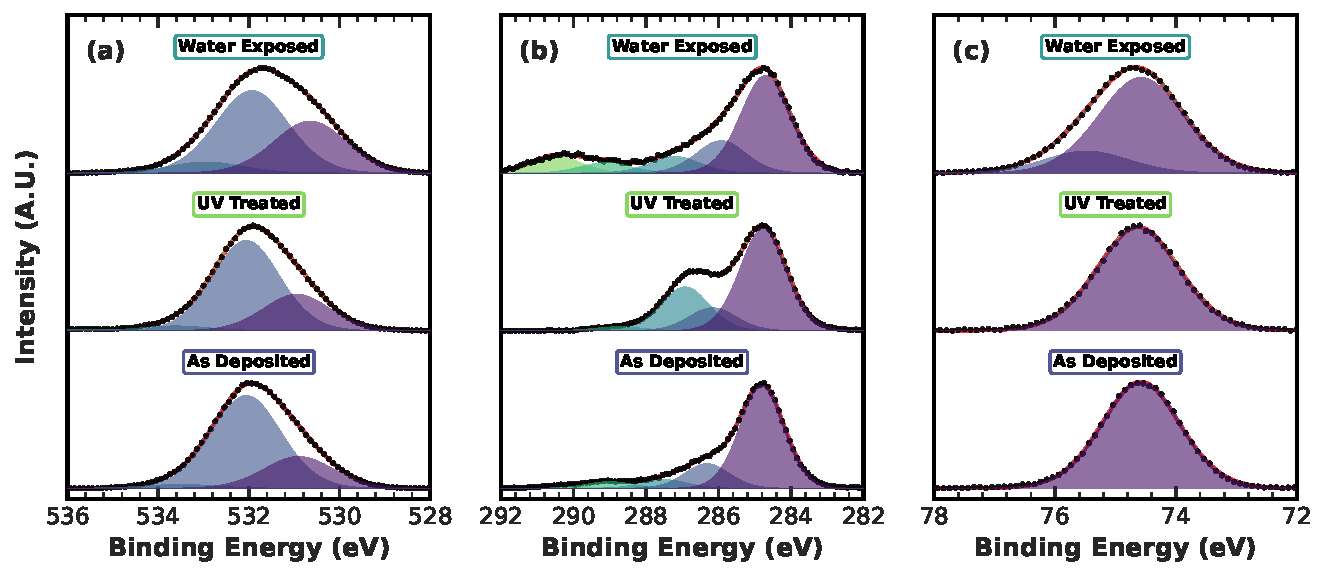
\includegraphics[width=0.95\textwidth]{Figures/XPS_publication_figure_final.pdf}
  \caption{High-resolution XPS spectra of BTY-based alucone films across as-deposited, water-exposed, and UV+water-exposed conditions. Columns show C~1s (left), O~1s (middle), and Al~2p (right) regions. Colored lines denote individual fit components; black crosses represent measured data.}
  \label{fig:xps_bty}
\end{figure}

\begin{figure}[H]
  \centering
  % \includegraphics[width=0.95\textwidth]{Figures/THB_XPS_Final_Publication.pdf}
  \begin{center}
    \fbox{\parbox{0.9\textwidth}{\centering\textbf{Placeholder: THB XPS Spectra}\\ High-resolution XPS for THB-based alucone films\\(C 1s, O 1s, Al 2p regions)}}
  \end{center}
  \caption{High-resolution XPS spectra of THB-based alucone films across as-deposited, water-exposed, and UV+water-exposed conditions. Columns show C~1s (left), O~1s (middle), and Al~2p (right) regions. Colored lines denote individual fit components; black crosses represent measured data.}
  \label{fig:xps_thb}
\end{figure}

\begin{table}[H]
\centering
\caption{Renormalized atomic \% (mean ± standard deviation) for O, C, and Al in TMA–BTY and TMA–THB alucone films across treatments. Ideal MLD values are calculated based on precursor stoichiometry.}
\label{tab:xps-bty-thb-corrected-final}
\begin{tabular}{l c c c c c c}
\toprule
\multirow{2}{*}{\textbf{Treatment}} & \multicolumn{3}{c}{\textbf{BTY [\%]}} & \multicolumn{3}{c}{\textbf{THB [\%]}} \\
\cmidrule(lr){2-4} \cmidrule(lr){5-7}
 & O & C & Al & O & C & Al \\
\midrule
As-Deposited & 29.2 ± 0.8 & 58.9 ± 0.4 & 11.9 ± 0.5 & 42.8 ± 1.8 & 25.9 ± 2.4 & 31.3 ± 0.6 \\
H$_2$O-Exposed & 56.0 ± 0.5 & 18.6 ± 0.5 & 25.3 ± 0.3 & 50.2 ± 0.6 & 17.2 ± 1.6 & 32.6 ± 1.0 \\
H$_2$O + UV & 32.9 ± 1.2 & 55.6 ± 1.5 & 11.5 ± 0.4 & 46.8 ± 1.0 & 20.2 ± 1.2 & 33.0 ± 0.1 \\
\midrule
Ideal (MLD) & 20.0 & 70.0 & 10.0 & 23.1 & 69.2 & 7.7 \\
\bottomrule
\end{tabular}
\end{table}

\subsection{Mechanistic Insight into UV-Induced Stabilization}

The combined spectroscopic evidence from FTIR and XPS supports a mechanistic model for UV-induced stabilization in TMA–BTY alucone films. Figure~\ref{fig:structure_evolution} schematically illustrates the proposed evolution from the as-deposited structure to a UV-crosslinked and chemically stabilized network.

As-deposited alucone films consist of alternating Al--O-- and organic segments formed from trimethylaluminum (TMA) and 1,4-butynediol (BTY), with a backbone structure nominally described as \ce{[-Al-O-CH2-C#C-CH2-O-]}. FTIR analysis reveals residual hydroxyl bands near 3622 and 3232~\si{\per\centi\meter}, indicating incomplete surface reactions or unreacted diol end-groups. XPS data further suggests a small population of methyl species (Al–C) likely originating from unreacted TMA ligands at the surface.

Upon UV exposure at \SI{254}{\nano\meter}, substantial chemical transformations occur. FTIR shows strong attenuation of O–H bands and the emergence of a sharp peak at \SI{1612}{\per\centi\meter}, indicative of conjugated C=C species. Concurrently, XPS reveals a significant increase in C=O contributions alongside a reduction in C–O intensity, implying cleavage of C–O bonds and oxidative rearrangement.

We propose that these spectral changes reflect a multi-step transformation initiated by UV-induced radical or [2+2] cycloaddition reactions between adjacent alkyne moieties. These reactions generate conjugated or aromatic domains and disrupt the original ether-like linkages. The newly formed C=O species likely arise from oxidation of alkyne-adjacent carbons, forming carbonyl-containing structures reminiscent of quinones. These conjugated C=C and C=O groups contribute to electron delocalization, stabilizing the hybrid network through aromatic or quasi-aromatic resonance.

This photochemical crosslinking is further supported by sharpening of fingerprint-region FTIR bands and retention of Al–O–C character in Al~2p and O~1s XPS spectra. The resulting structure is chemically denser, less permeable to water, and resistant to hydrolysis. By contrast, non-irradiated films show pronounced degradation under aqueous exposure, with loss of carbon and formation of hydrolyzed Al–O–Al species.

While THB-based alucone films also showed modest UV-induced stabilization and good intrinsic resistance to hydrolysis, their spectroscopic profiles revealed only subtle changes upon irradiation, with minimal evidence of crosslinking or new conjugated features. The absence of significant C=O growth or structural reorganization suggests limited potential for negative-tone resist behavior, where crosslinking and developer resistance are essential. Consequently, BTY-based alucones were selected as the lead candidate for electron-beam lithography evaluation, owing to their pronounced photochemical reactivity and structural transformation upon UV exposure.

\begin{figure}[ht]
  \centering
  % \includegraphics[width=0.85\textwidth]{figures/structure_evolution.pdf}
  \begin{center}
    \fbox{\parbox{0.8\textwidth}{\centering\textbf{Placeholder: Structure Evolution Figure}\\ Schematic showing proposed UV-induced crosslinking mechanism}}
  \end{center}
  \caption{Proposed structural evolution and chemical transformations of BTY-based alucone films during UV irradiation and subsequent hydrolytic exposure: (a) as-deposited film containing residual hydroxyl groups and isolated alkyne linkages, (b) UV-treated film exhibiting crosslinked conjugated structures and reduced hydroxyl content, and (c) hydrolytically degraded film without UV treatment, illustrating extensive bond cleavage and porous structure formation.}
  \label{fig:structure_evolution}
\end{figure}


\subsection{Electron-Beam Lithography Studies}

The lithographic performance of BTY-based alucone films was evaluated using electron-beam lithography (EBL) on a JEOL JBX-6300FS system operating at \SI{100}{\kilo\volt}. Films were flood-exposed to UV light prior to EBL to initiate partial crosslinking, as established in previous sections.

A dose matrix was patterned onto the films and developed in \SI{0.01}{\molar} HCl for \SI{10}{\second}. Well-defined square features were observed across a dose range of \SIrange{500}{2000}{\micro\coulomb\per\centi\meter\squared}. Above \SI{2000}{\micro\coulomb\per\centi\meter\squared}, haloing effects became apparent at feature boundaries, attributed to electron scattering and proximity effects, resulting in excess material retention beyond the intended dose region.

Profilometry measurements were performed across individual squares to quantify retained film thickness as a function of dose. These data confirmed a negative-tone resist response, with increasing thickness corresponding to increasing dose up to saturation. Step height measurements will be used to extract contrast and dose-to-clear values (Figure~\ref{fig:contrast_curve_placeholder}).

Atomic force microscopy (AFM) was used to characterize the edges and corners of squares within the optimal dose range. These scans revealed sharp edge definition, minimal roughness, and flat residual film topography, consistent with clean pattern transfer and uniform development. Representative AFM images and surface height profiles are shown in Figure~\ref{fig:afm_corner_placeholder}. Full surface maps and extended profiles are included in the Supplementary Information.

A second pattern consisting of box and grating features was exposed using the optimal dose identified from the matrix. Scanning electron microscopy (SEM) and AFM imaging of these features are being used to evaluate resolution, line edge roughness (LER), and three-dimensional profile fidelity. Together, these measurements establish BTY-based alucone as a negative-tone hybrid resist with robust developer contrast, submicron pattern resolution, and compatibility with acidic development.

\begin{figure}[ht]
  \centering
  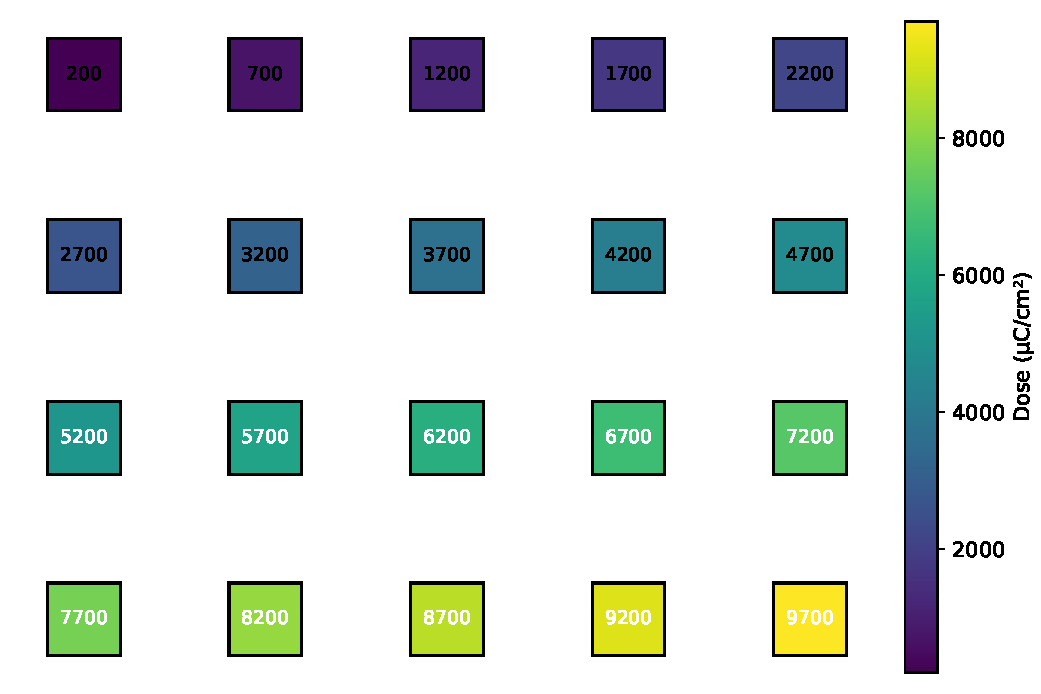
\includegraphics[width=0.75\textwidth]{Figures/dose_matrix_mockup_clean.pdf}
  \caption{Dose matrix layout and representative square features used to evaluate lithographic contrast in BTY-based alucone films. Step height data across each square was used to generate a contrast curve. Final figure will include profilometry overlay.}
  \label{fig:contrast_curve_placeholder}
\end{figure}

\begin{figure}[ht]
  \centering
  % \includegraphics[width=0.75\textwidth]{Figures/DR_250501_AluconeBTY_Sampe6_corner.500_00003_1.smp.png}
  \begin{center}
    \fbox{\parbox{0.7\textwidth}{\centering\textbf{Placeholder: AFM Image}\\ AFM topography of patterned features\\(3D surface profile)}}
  \end{center}
  \caption{AFM image of the corner of a BTY-based alucone square developed after EBL exposure at the optimal dose. Sharp corner retention and flat film interior indicate effective negative-tone patterning. Surface map and line profile shown.}
  \label{fig:afm_corner_placeholder}
\end{figure}

\subsubsection{SEM}
SEM imaging was carried out on the dose matrix consisting of 100 µm × 100 µm square patterns with doses ranging from 100 to 30,000 µC/cm². Additionally, fine feature matrices were imaged to assess resolution capabilities.

\subsubsection{Dose Matrices and Contrast Curve Analysis}
Contrast curves were generated from both SEM and AFM measurements to characterize the resist response across different developers. The normalized thickness data revealed distinct crosslinking and graphitization regions, necessitating a segmented fitting approach.

For the crosslinking region (low to moderate doses), a sigmoid function was fitted:
\begin{equation}
f(D) = \frac{1}{1 + (D_{50}/D)^{\gamma}}
\end{equation}
where $D_{50}$ is the dose at 50\% normalized thickness and $\gamma$ is the contrast parameter.

For the graphitization region (high doses), a linear decay function was applied:
\begin{equation}
f(D) = \text{slope} \times D + \text{intercept}
\end{equation}

The AFM measurements on 2 µm line gratings (1 µm gap) showed similar behavior, with thickness increasing to a peak followed by reduction at high doses. The average contrast across all developers was $\gamma = 2.54$, with individual values of:
\begin{itemize}
    \item 0.005M HCl 10s: $\gamma = 0.91$, $D_{50} = 1225.1$ µC/cm²
    \item 0.01M HCl 10s: $\gamma = 3.25$, $D_{50} = 9223.7$ µC/cm²
    \item 0.01M HCl 5s: $\gamma = 3.44$, $D_{50} = 2447.5$ µC/cm²
\end{itemize}

Notably, the two 0.01M developers exhibited similar high contrast values ($\gamma \approx 3.3-3.4$), as expected for identical developer concentrations, while the 0.005M developer showed significantly lower contrast ($\gamma = 0.91$). The 0.01M HCl 10s sample showed no thickness reduction even at the highest doses (30,000 µC/cm²), suggesting incomplete graphitization under these development conditions. In contrast, both the 0.005M 10s and 0.01M 5s samples exhibited clear decay regions above their respective peak doses (3000 and 7000 µC/cm²).

The SEM-based contrast curve (Figure X) showed good agreement with the AFM data, with a clear transition at approximately 3958 µC/cm² between the crosslinking and graphitization regions. The normalized SEM gray values demonstrated the expected sigmoid behavior in the crosslinking region, transitioning to exponential decay at high doses as the resist underwent densification and carbonization.
